\documentclass[11pt]{article}

\usepackage[margin=1in]{geometry}
\usepackage{amsmath,amssymb,amsthm}
\usepackage{enumitem}
\usepackage{graphicx}
\usepackage[hidelinks]{hyperref}

\newtheorem{theorem}{Theorem}
\newtheorem{corollary}{Corollary}

\newcommand{\Ext}{\operatorname{Ext}}
\newcommand{\dist}{\operatorname{dist}}
\newcommand{\id}{\operatorname{id}}
\newcommand{\R}{\mathbb{R}}

\title{A Uniform Ext Constant for Normalized Exact Sequences}
\author{arXiv automatic math run \texttt{fa\_banach\_001}}
\date{Candidate packet, June 14, 2026}

\begin{document}
\maketitle

\section*{Classification}

\begin{itemize}[leftmargin=2em]
\item \textbf{Status:} conditional / normalized exact-sequence result.
\item \textbf{Source:} P. Kochanek, \emph{Stability of vector measures and
twisted sums of Banach spaces}, arXiv:1208.4755.
\item \textbf{Target:} final Problem (6), asking whether the property
$\Ext(\mathfrak X,\cdot)=0$ is a uniform three-space property.
\end{itemize}

\section*{Source Question}

The source paper asks whether there is a function
\[
\varphi:(0,\infty)^2\longrightarrow (0,\infty)
\]
such that, whenever $\mathfrak X,X,Y,Z$ are Banach spaces,
$0\to Y\to Z\to X\to 0$ is exact, and
$\Ext(\mathfrak X,X)=0=\Ext(\mathfrak X,Y)$, then
\[
\Ext(\mathfrak X,Z)=0
\quad\text{and}\quad
Z(\mathfrak X,Z)\leq
\varphi\bigl(Z(\mathfrak X,X),Z(\mathfrak X,Y)\bigr).
\]
Here $Z(U,V)$ is the best constant for approximating zero-linear maps
$U\to V$ by linear maps, as in the source paper.

\begin{center}
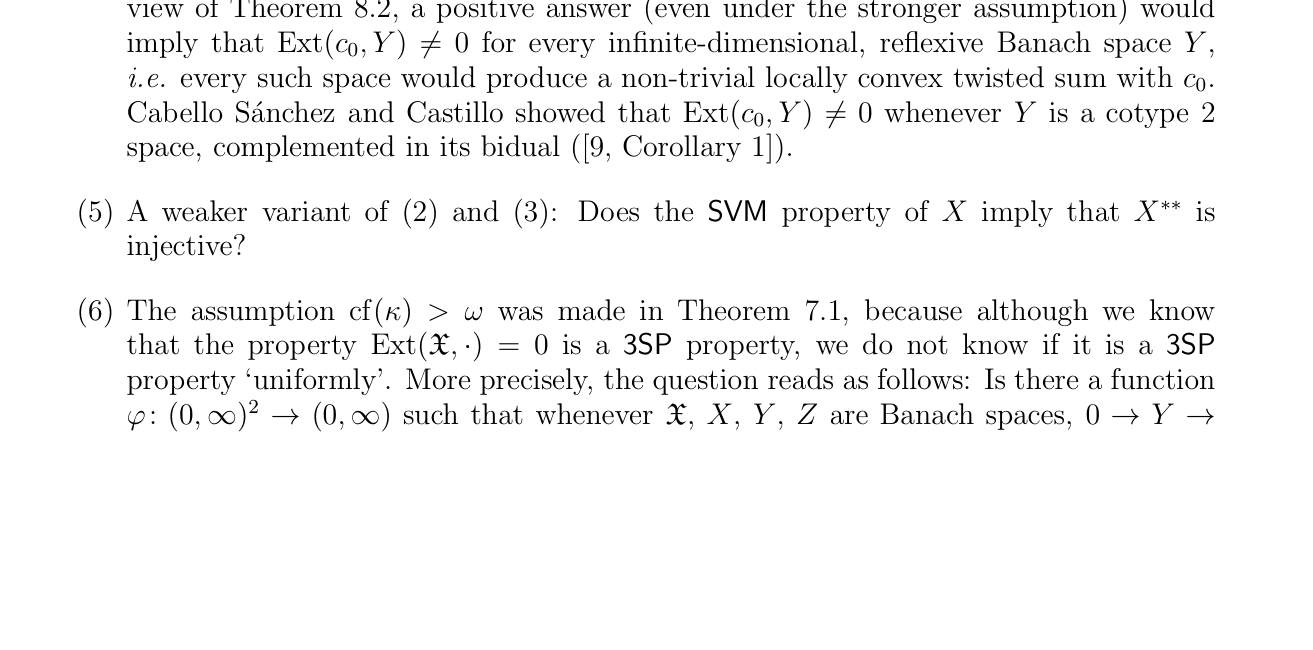
\includegraphics[width=\linewidth]{figures/open_problem_page37_bottom.png}

\vspace{0.5em}

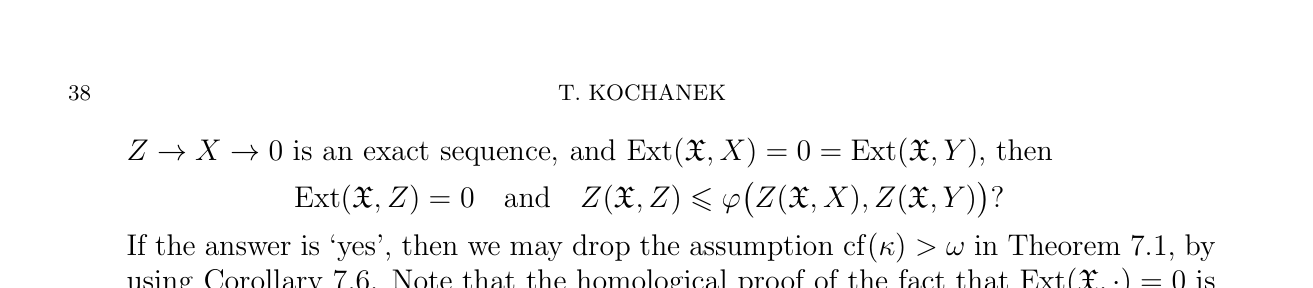
\includegraphics[width=\linewidth]{figures/open_problem_page38_top.png}
\end{center}

\section*{Conditional Dependencies}

The theorem below is proved for exact sequences in the following normalized
form.  We assume that
\[
0\longrightarrow Y \xrightarrow{j} Z \xrightarrow{q} X\longrightarrow 0
\]
has isometric kernel inclusion and admits a homogeneous right inverse
$b:X\to Z$ of $q$ such that
\[
q b=\id_X,\qquad \|b(x)\|\leq s\|x\|\quad (x\in X).
\]
This is automatic, for every $s>1$, in the canonical metric-quotient model
where $Y$ is a closed subspace of $Z$, $X=Z/Y$ has the quotient norm, and $q$
is the quotient map.

Thus, if the source question is interpreted in this normalized model, the
corollary gives an affirmative bound. If the question is interpreted literally
for arbitrary endpoint identifications in exact sequences, this packet leaves
one dependency: the quotient open-map and embedding distortion constants would
also have to be controlled, or shown irrelevant, using only
$Z(\mathfrak X,X)$ and $Z(\mathfrak X,Y)$.

\section*{Proof Intuition}

Let $F:E\to Z$ be zero-linear. Push $F$ down to the quotient $X$ and use
$Z(E,X)$ to straighten $qF$ by a linear map.  Lift that linear map
algebraically back to $Z$; boundedness is not needed because linear
approximants in the zero-linear definition are not required to be continuous.
After subtracting the lift, the remaining map has small quotient part.  A
homogeneous selector lifts this small quotient part back into $Z$; subtracting
it leaves a zero-linear map into the kernel $Y$.  Applying $Z(E,Y)$ to this
kernel-valued map finishes the approximation.  The only constant loss comes
from lifting the quotient error through the selector.

\section*{Theorem}

\begin{theorem}
Let $E,X,Y,Z$ be Banach spaces and suppose that
\[
0\longrightarrow Y \xrightarrow{j} Z \xrightarrow{q} X\longrightarrow 0
\]
is exact, $j$ is an isometry onto $\ker q$, $\|q\|\leq 1$, and $q$ has a
homogeneous right inverse $b:X\to Z$ satisfying
\[
q b=\id_X,\qquad \|b(x)\|\leq s\|x\|\quad (x\in X).
\]
Put $A=Z(E,X)$ and $B=Z(E,Y)$, allowing $A$ or $B$ to be $+\infty$.  If
$A,B<\infty$, then
\[
Z(E,Z)\leq sA+B(1+2sA).
\]
\end{theorem}

\begin{proof}
Let $F:E\to Z$ be zero-linear and write $\delta=Z(F)$. If $\delta=0$, the
same argument below applies with every estimate equal to $0$, so assume
$\delta>0$.

Since $\|q\|\leq 1$, the composition $qF:E\to X$ is zero-linear and
$Z(qF)\leq \delta$.  By the definition of $A$, for every $\varepsilon>0$
there is a linear map $\ell:E\to X$ such that
\[
\dist(qF,\ell)\leq (A+\varepsilon)\delta.
\]
Choose an algebraic linear lift $L:E\to Z$ of $\ell$, so that $qL=\ell$.
No boundedness of $L$ is required.  Set
\[
G=F-L,\qquad u=qG=qF-\ell.
\]
Then $G$ is zero-linear with $Z(G)=\delta$, and by homogeneity
\[
\|u(x)\|\leq (A+\varepsilon)\delta \|x\| \qquad (x\in E).
\]

Define
\[
H=G-bu.
\]
Because $qb=\id_X$, we have $qH=0$, hence $H(E)\subseteq j(Y)$.  Identifying
$Y$ with $j(Y)$, we estimate the zero-linearity of $H$. For any finite family
$x_1,\ldots,x_n\in E$,
\[
\begin{aligned}
&\left\|H\left(\sum_i x_i\right)-\sum_i H(x_i)\right\|\\
&\quad\leq
\left\|G\left(\sum_i x_i\right)-\sum_iG(x_i)\right\|
+\left\|b u\left(\sum_i x_i\right)-\sum_i b u(x_i)\right\|\\
&\quad\leq
\delta\sum_i\|x_i\|
+s\left\|u\left(\sum_i x_i\right)\right\|
+s\sum_i\|u(x_i)\|\\
&\quad\leq
\bigl(1+2s(A+\varepsilon)\bigr)\delta\sum_i\|x_i\|.
\end{aligned}
\]
Thus $H$ is a $Y$-valued zero-linear map with
\[
Z(H)\leq \bigl(1+2s(A+\varepsilon)\bigr)\delta.
\]
By the definition of $B$, for every $\eta>0$ there is a linear
$m:E\to Y$ satisfying
\[
\dist(H,jm)\leq
(B+\eta)\bigl(1+2s(A+\varepsilon)\bigr)\delta.
\]
Then $L+jm:E\to Z$ is linear, and for $\|x\|\leq 1$,
\[
\begin{aligned}
\|F(x)-(L+jm)(x)\|
&=\|G(x)-jm(x)\|\\
&\leq \|H(x)-jm(x)\|+\|b u(x)\|\\
&\leq
(B+\eta)\bigl(1+2s(A+\varepsilon)\bigr)\delta
+s(A+\varepsilon)\delta .
\end{aligned}
\]
Taking the infimum over admissible linear approximants and then letting
$\varepsilon,\eta\downarrow 0$ gives
\[
Z(E,Z)\leq sA+B(1+2sA).
\]
\end{proof}

\begin{corollary}
In the canonical metric-quotient normalization
$0\to Y\to Z\to Z/Y\to 0$,
\[
Z(E,Z)\leq Z(E,Z/Y)+Z(E,Y)+2Z(E,Z/Y)Z(E,Y).
\]
Consequently, for a normalized exact sequence
$0\to Y\to Z\to X\to 0$ with $X$ carrying the quotient norm,
\[
\varphi(a,b)=a+b+2ab
\]
is an admissible uniform three-space bound.
\end{corollary}

\begin{proof}
For each $s>1$, the quotient map admits a homogeneous selection
$b:X\to Z$ with $\|b(x)\|\leq s\|x\|$: choose, for each non-zero ray in $X$,
a representative within the factor $s$ of the quotient norm and extend
homogeneously.  Apply the theorem and let $s\downarrow 1$.
\end{proof}

\section*{Verification and Novelty Notes}

The proof uses only the definitions of zero-linear maps, the stability
constant $Z(E,\cdot)$, and the standard homogeneous selection for a quotient
map. The linear lift $L$ is purely algebraic, which is legitimate because the
linear maps used in the definition of $Z(E,V)$ need not be bounded.

The bounded novelty check for this packet searched the run registry and
solution/attempt indexes for arXiv:1208.4755 and for the core phrases
``uniform 3SP'', ``zero-linear'', and ``$Z(E,Z)$''.  No existing packet or
attempt for this exact target was found.  Short phrase searches for the
displayed bound and the source problem did not reveal an obvious literature
duplicate.  The result is therefore recorded as a candidate new
conditional/normalized estimate, not as a claimed full answer under every
possible interpretation of the source question.

\section*{Human Review Recommendation}

Reviewers should first decide whether Kochanek's final question is intended
only up to the canonical quotient normalization.  If yes, the corollary appears
to give a direct affirmative answer with
\[
\varphi(a,b)=a+b+2ab.
\]
If arbitrary endpoint identifications are part of the intended formulation,
the reviewer should test whether the missing quotient and embedding distortion
constants can be absorbed by the endpoint stability constants alone.

\begin{thebibliography}{9}

\bibitem{kochanek}
P. Kochanek,
\emph{Stability of vector measures and twisted sums of Banach spaces},
arXiv:1208.4755.

\bibitem{cabello-castillo}
F. Cabello Sanchez and J. M. F. Castillo,
\emph{Stability constants and the homology of quasi-Banach spaces},
Israel J. Math. 198 (2013), 347--370.

\end{thebibliography}

\end{document}
